% Chapter Template

\chapter{Ensayos y Resultados} % Main chapter title
\label{Chapter4}

En este capítulo se detallan las pruebas efectuadas sobre el hardware y el firmware a lo largo del desarrollo y se analizan los resultados obtenidos.
 
\section{Pruebas de concepto}
\label{sec:PruebasConcepto}

Para determinar la factibilidad de los objetivos planteados en la sección \ref{sec:objetivos} y poder, al mismo tiempo, cumplir con los requerimientos funcionales detallados en la sección \ref{sub:Requisitos}, se implementó en la primera etapa del proyecto un modelo destinado validar todas las suposiciones efectuadas en el diseño preliminar. Para esto se utilizó una placa de evaluación ESP32-DEVKITC-32D-F\cite{noauthor_esp32-devkitc_nodate} ofrecida por la firma Expressif, pensada para facilitar este tipo de procesos. Usando esta placa como núcleo, se construyó en forma cableada una maqueta de lo que sería el equipo definitivo. Una versión de este montaje puede observase en la figura \ref{fig:Demostrador}.

\begin{figure}[ht]
	\centering
	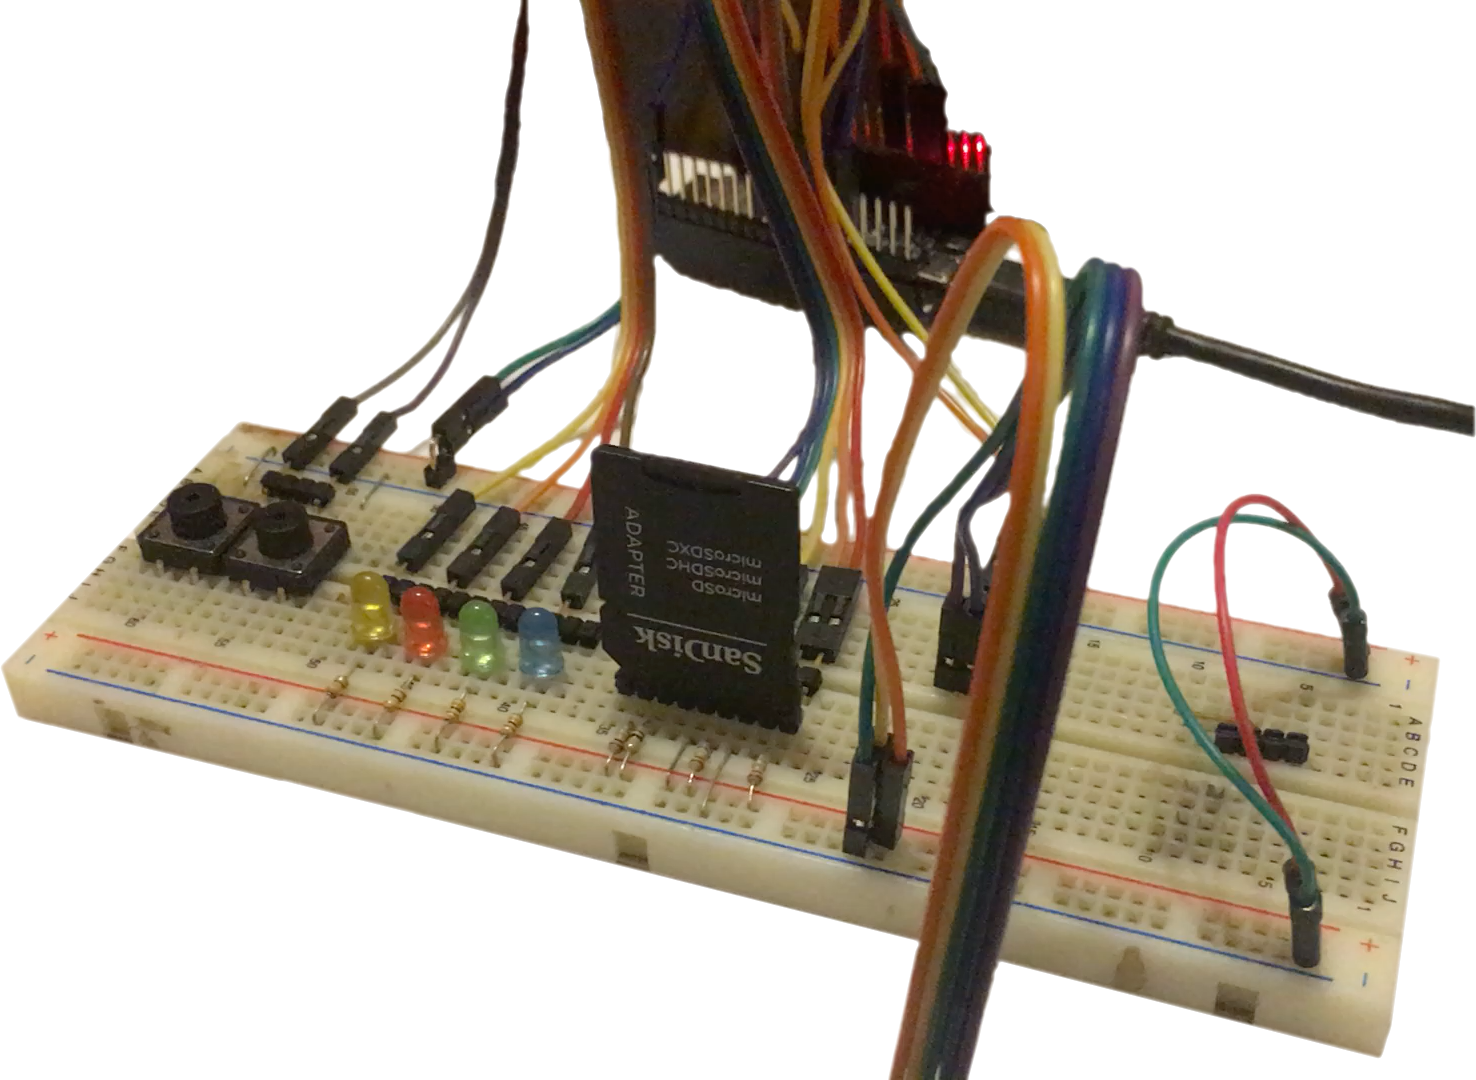
\includegraphics[width=0.8\textwidth]{Figures/Demostrador.png}
	\caption[Montaje utilizado para las pruebas de concepto]{Imagen con el montaje de componentes en torno a la placa de evaluación utilizado para la prueba de concepto.}
	\label{fig:Demostrador}
\end{figure}

De forma similar, utilizando los ejemplos de software provisto por el fabricante en el ESP-IDF\cite{noauthor_esp-idf_nodate}\cite{noauthor_espressifesp-idf_2020}, se empezaron a estudiar y probar las bibliotecas de software que se utilizarían en el desarrollo. Así se pudo validar cada uno de los bloques del código, para empezar a integrarlos en lo que sería la primera versión del firmware definitivo. 

Como resultado de este proceso se obtuvo una primera versión del equipo que podía leer una tarjeta de proximidad, determinar la fecha y hora mediante un RTC, escribir en una tarjeta de memoria microSD el identificador de la etiqueta RFID leída junto con la fecha y hora del evento, y transmitir esta información mediante WiFi a una computadora.

\section{Pruebas funcionales del hardware}
\label{sec:pruebasHW}

La fabricación del prototipo de hardware se dividió en dos etapas: primero se montaron todos los componentes correspondientes a la etapa de alimentación del equipo para verificar que todas las tensiones generadas fueran correctas. A continuación se montaron el resto de los componentes, y se verificó, en forma ordenada, el correcto funcionamiento de cada uno utilizando las siguientes pruebas:

\begin{enumerate}
	\item Para verificar el funcionamiento del procesador se lo configuró para iniciar en modo \emph{bootloader} y grabarle un programa de prueba. De esta forma se determinó que el procesador no completaba el proceso de \emph{reset} porque faltaba una resistencia de \emph{pull-up} en el terminal de \emph{Enable}. Para resolver este problema se agregó la resistencia R27, que se puede ver en la figura \ref{fig:ErroresPrototipo}.
	
	\item Continuando con la verificación del procesador, se lo configuró para iniciar en modo normal y ejecutar el programa cargado en el apartado anterior. Durante esta prueba se determinó que el procesador no podía iniciar en modo normal porque faltaba una resistencia de \emph{pull-up} en el terminal que determina el modo de arranque. Para resolver este problema se agregó la resistencia R28, que se puede ver en la figura \ref{fig:ErroresPrototipo}.
	
\begin{figure}[ht]
	\centering
	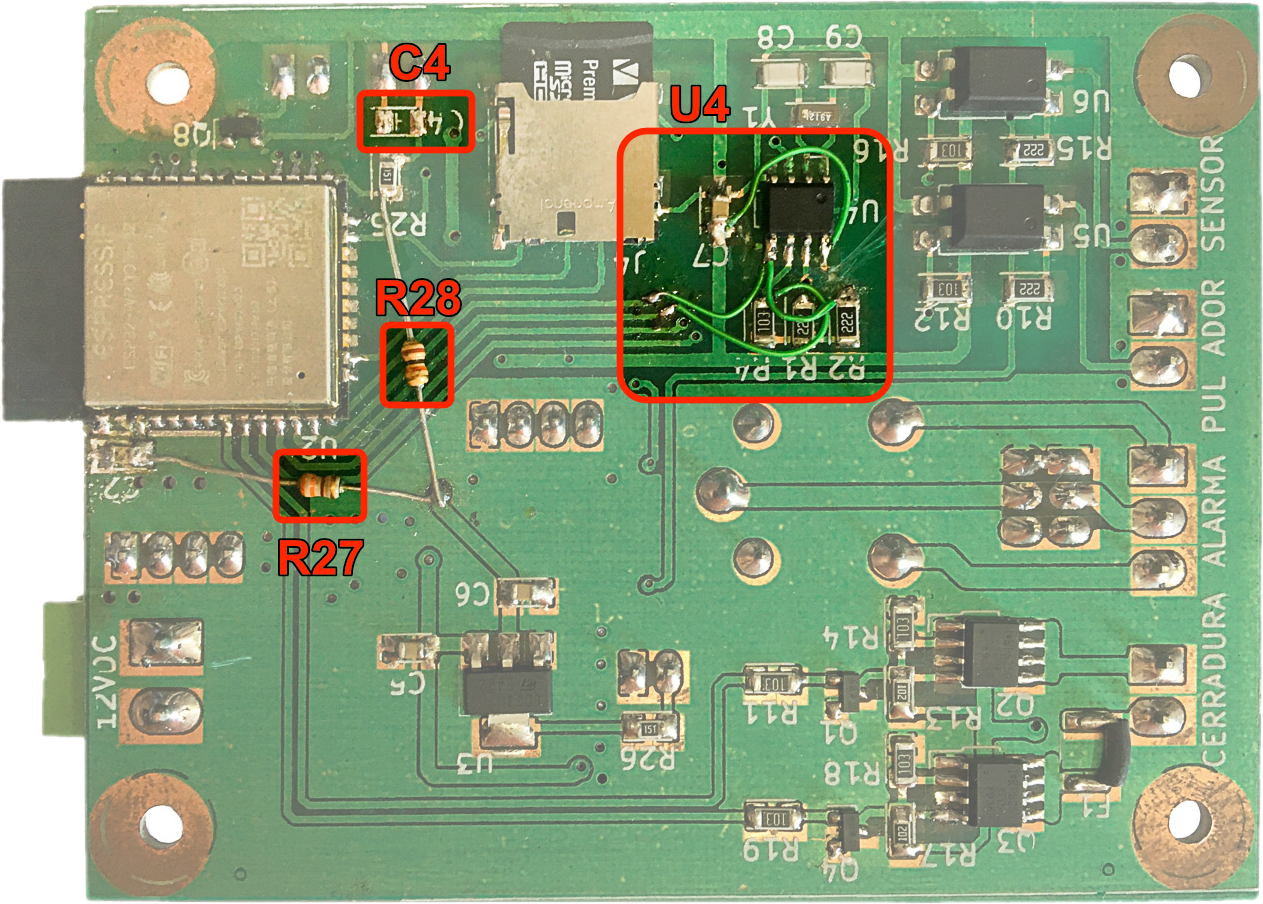
\includegraphics[width=0.9\textwidth]{Figures/LadoSoldadura.png}
	\caption[Errores detectados durante el montaje del prototipo]{Imagen con las correcciones efectuadas en el prototipo para resolver los errores detectados durante el montaje.}
	\label{fig:ErroresPrototipo}
\end{figure}

	\item Con el procesador en funcionamiento, se probaron las entradas y salidas digitales con programas simples que activan una salida como respuesta a un cambio en una entrada. Para facilitar la identificación de las causas de los problemas, todos estos programas de prueba utilizaron las funciones de consola disponibles en este procesado. De esta forma se pueden ver en una consola serial de la computadora de desarrollo mensajes generados en el programa del procesador embebido utilizando el mismo puerto de comunicaciones por el que se realizan los cambios de firmware.
	
	\item Para verificar el funcionamiento de la tarjeta microSD y el sistema de archivos se utilizó un programa de prueba simple para crear un archivo y almacenar en él una cadena de texto. Para certificar que funcionamiento fuese correcto se retiró la tarjeta de memoria del equipo y se comprobó el contenido del archivo en una computadora.
	
	\item Para verificar la comunicación con el circuito integrado responsable de la lectura de las tarjetas de proximidad se utilizó directamente la maqueta del firmware desarrollada en las pruebas de concepto. Tampoco se encontraron inconvenientes en la comunicación con la lectora de proximidad en el prototipo de hardware.
	
	\item Para verificar el funcionamiento del RTC también se recurrió a la maqueta del firmware utilizada en las pruebas del apartado anterior. En este caso se encontró un error importante en las conexiones del circuito integrado, originado por un error en la numeración de los terminales al definir el componente en Kicad, el programa donde se realizó el diseño de toda la placa electrónica. Este error se puede apreciar en la figura \ref{fig:ErrorRTC}, al comparar la información correspondiente a la hoja de datos\cite{noauthor_mcp7940n_nodate}, en la mitad izquierda de la figura, con la definición del componente, ubicada en la mitad derecha, vemos que todos los terminales del lado derecho se encuentran invertidos. En la figura \label{fig:ErroresPrototipo} se pueden observar las correcciones efectuadas sobre el prototipo para subsanar este problema.
	
\begin{figure}[ht]
	\centering
	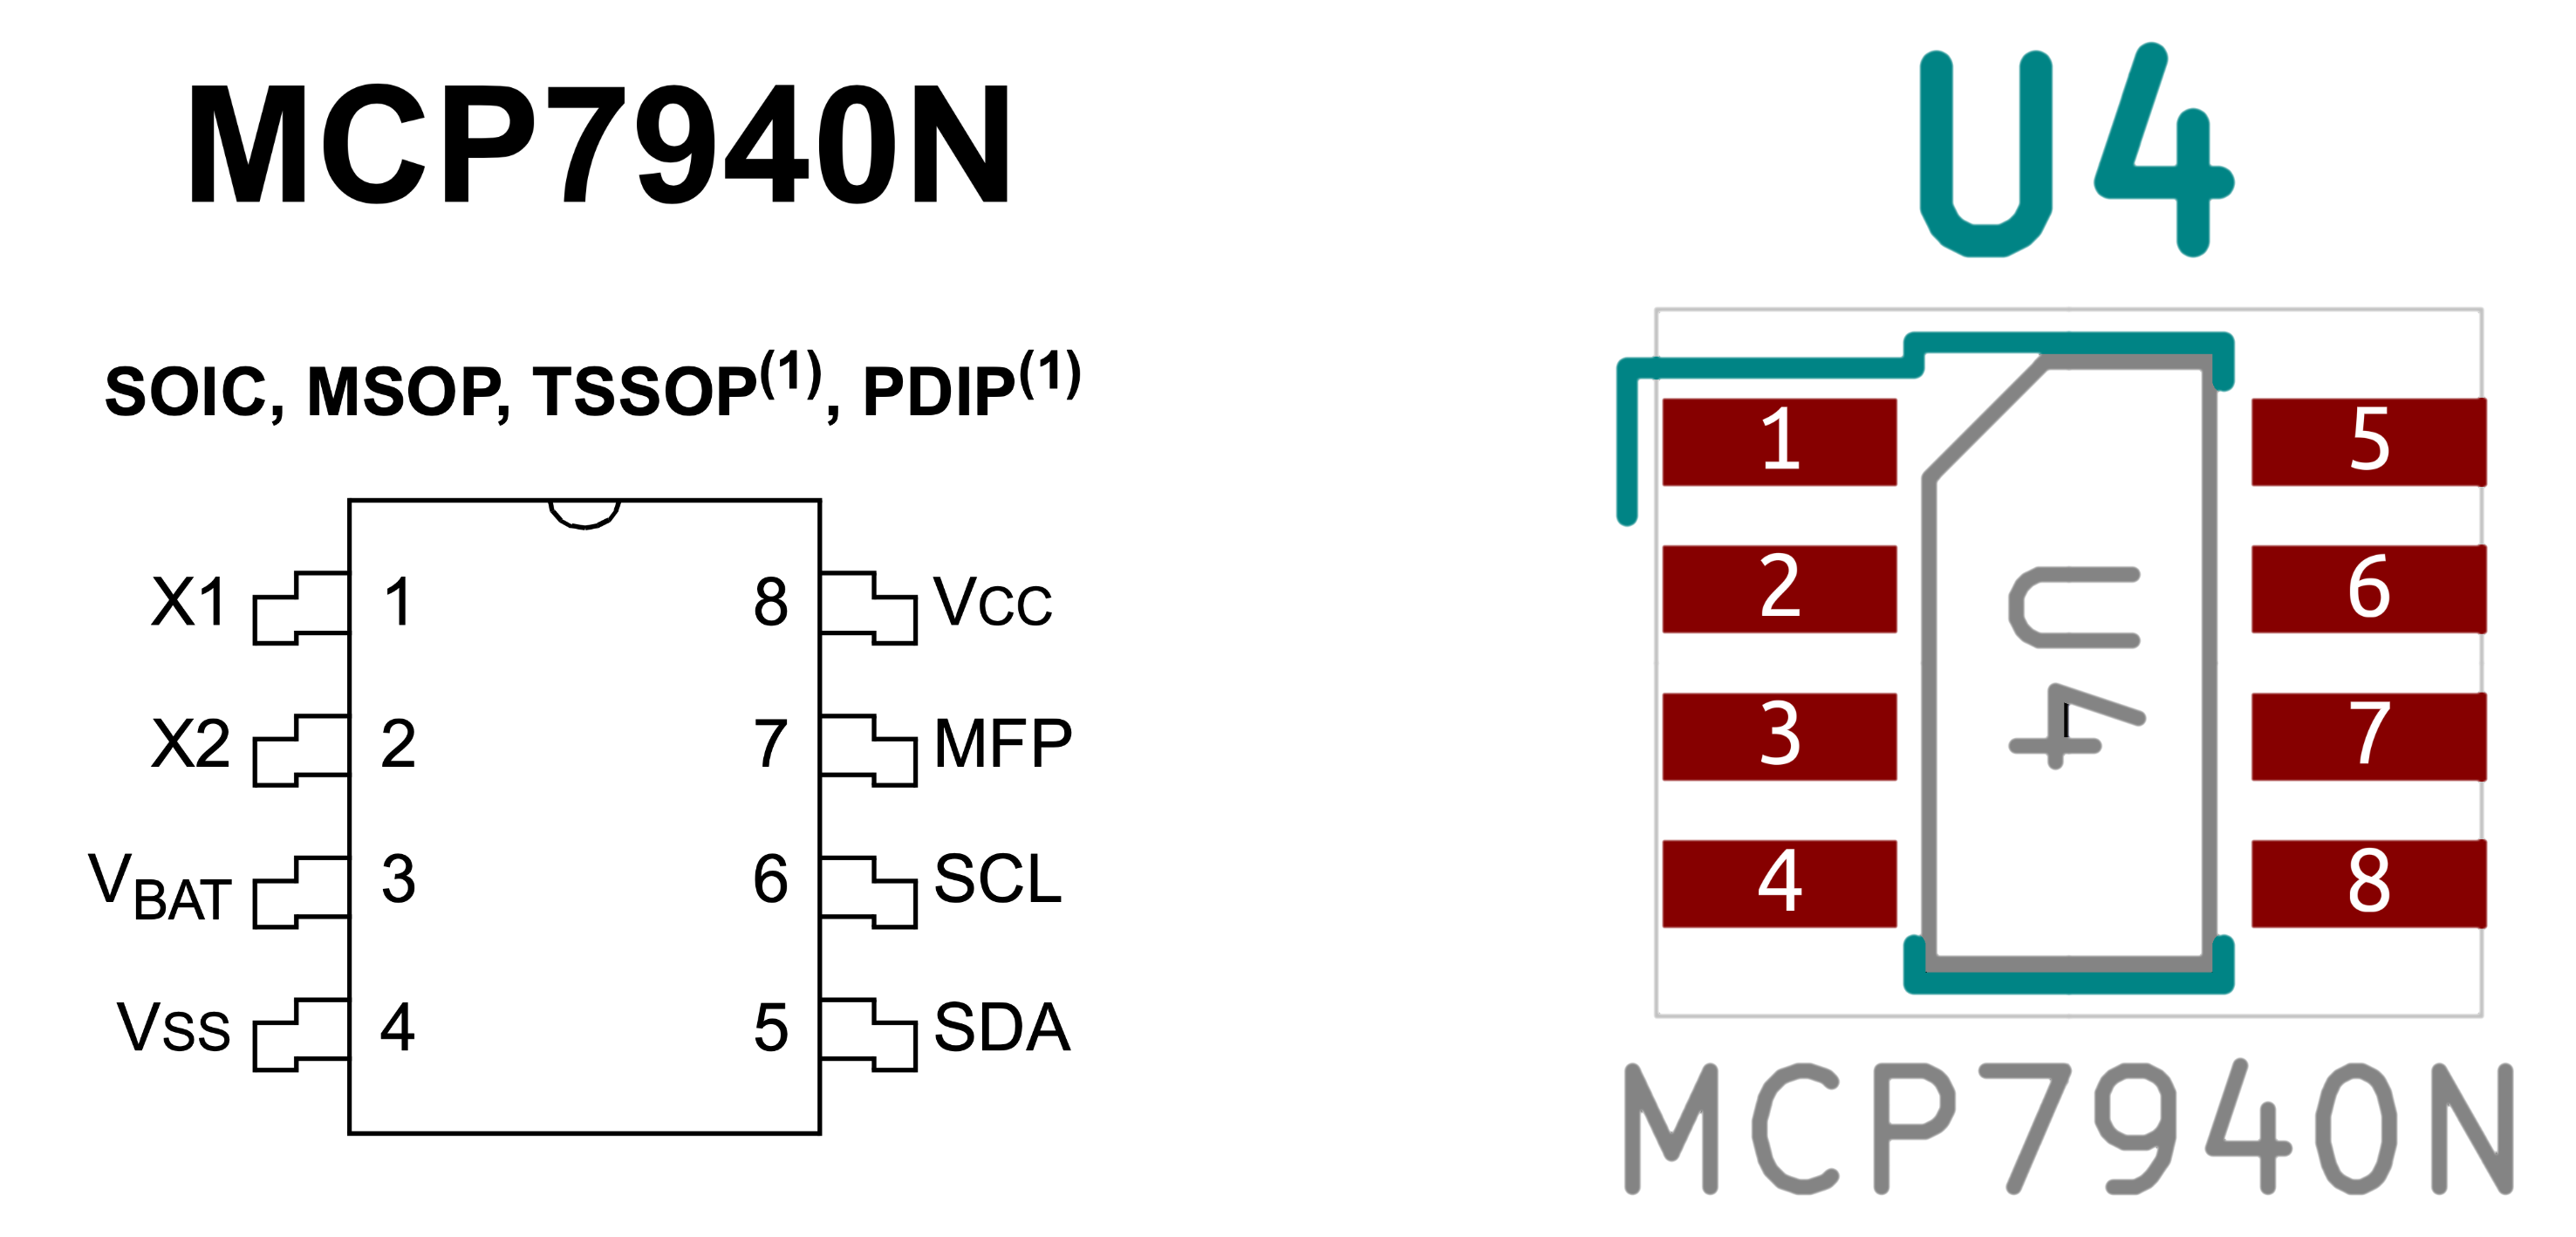
\includegraphics[width=0.9\textwidth]{Figures/ErrorHuella.png}
	\caption[Error en la asignacion de terminales del RTC]{Imagen que compara la asignación de terminales del RTC según la hoja de datos, a la izquierda, con la efectuada en la huella del componente Kicad.}
	\label{fig:ErrorRTC}
\end{figure}

	\item Finalmente, a lo largo de los sucesivos reinicios de la placa se determinó que al conectar la alimentación del equipo, el procesador inciaba en modo \emph{bootloader} en lugar de ejecutar el programa ya grabado. Se comprobó también que esto no sucedía al efectuar un \emph{reset} sin interrumpir la alimentación del equipo. Se determinó al capacitor C4 como el responsable y se removió del diseño, como se puede observar en la figura \label{fig:ErroresPrototipo}.
\end{enumerate}

\FloatBarrier

\section{Pruebas unitarias y de integración}
\label{sec:PruebasFirmware}

Como ya se explicó en la sección \ref{sec:desarrollo} todo el desarrollo del firmware se planteó utilizando la metodología TDD. Esto implica que se escribieron pruebas unitarias y de integración para la mayoría de los componentes de software desarrollados. Una forma cuantitativa de evaluar estas pruebas son los informes de cobertura generados Ceedling, la herramienta utilizada para ejecutar las pruebas automatizadas y consolidar los resultados. En la figura \ref{fig:Cobertura} se puede observar el informe de cobertura, donde se puede apreciar que las pruebas automatizadas ejecutan casi del 95\% de las líneas de código escritas y explora más del 80\% de las combinaciones en los saltos condicionales.

\begin{figure}[ht]
	\centering
	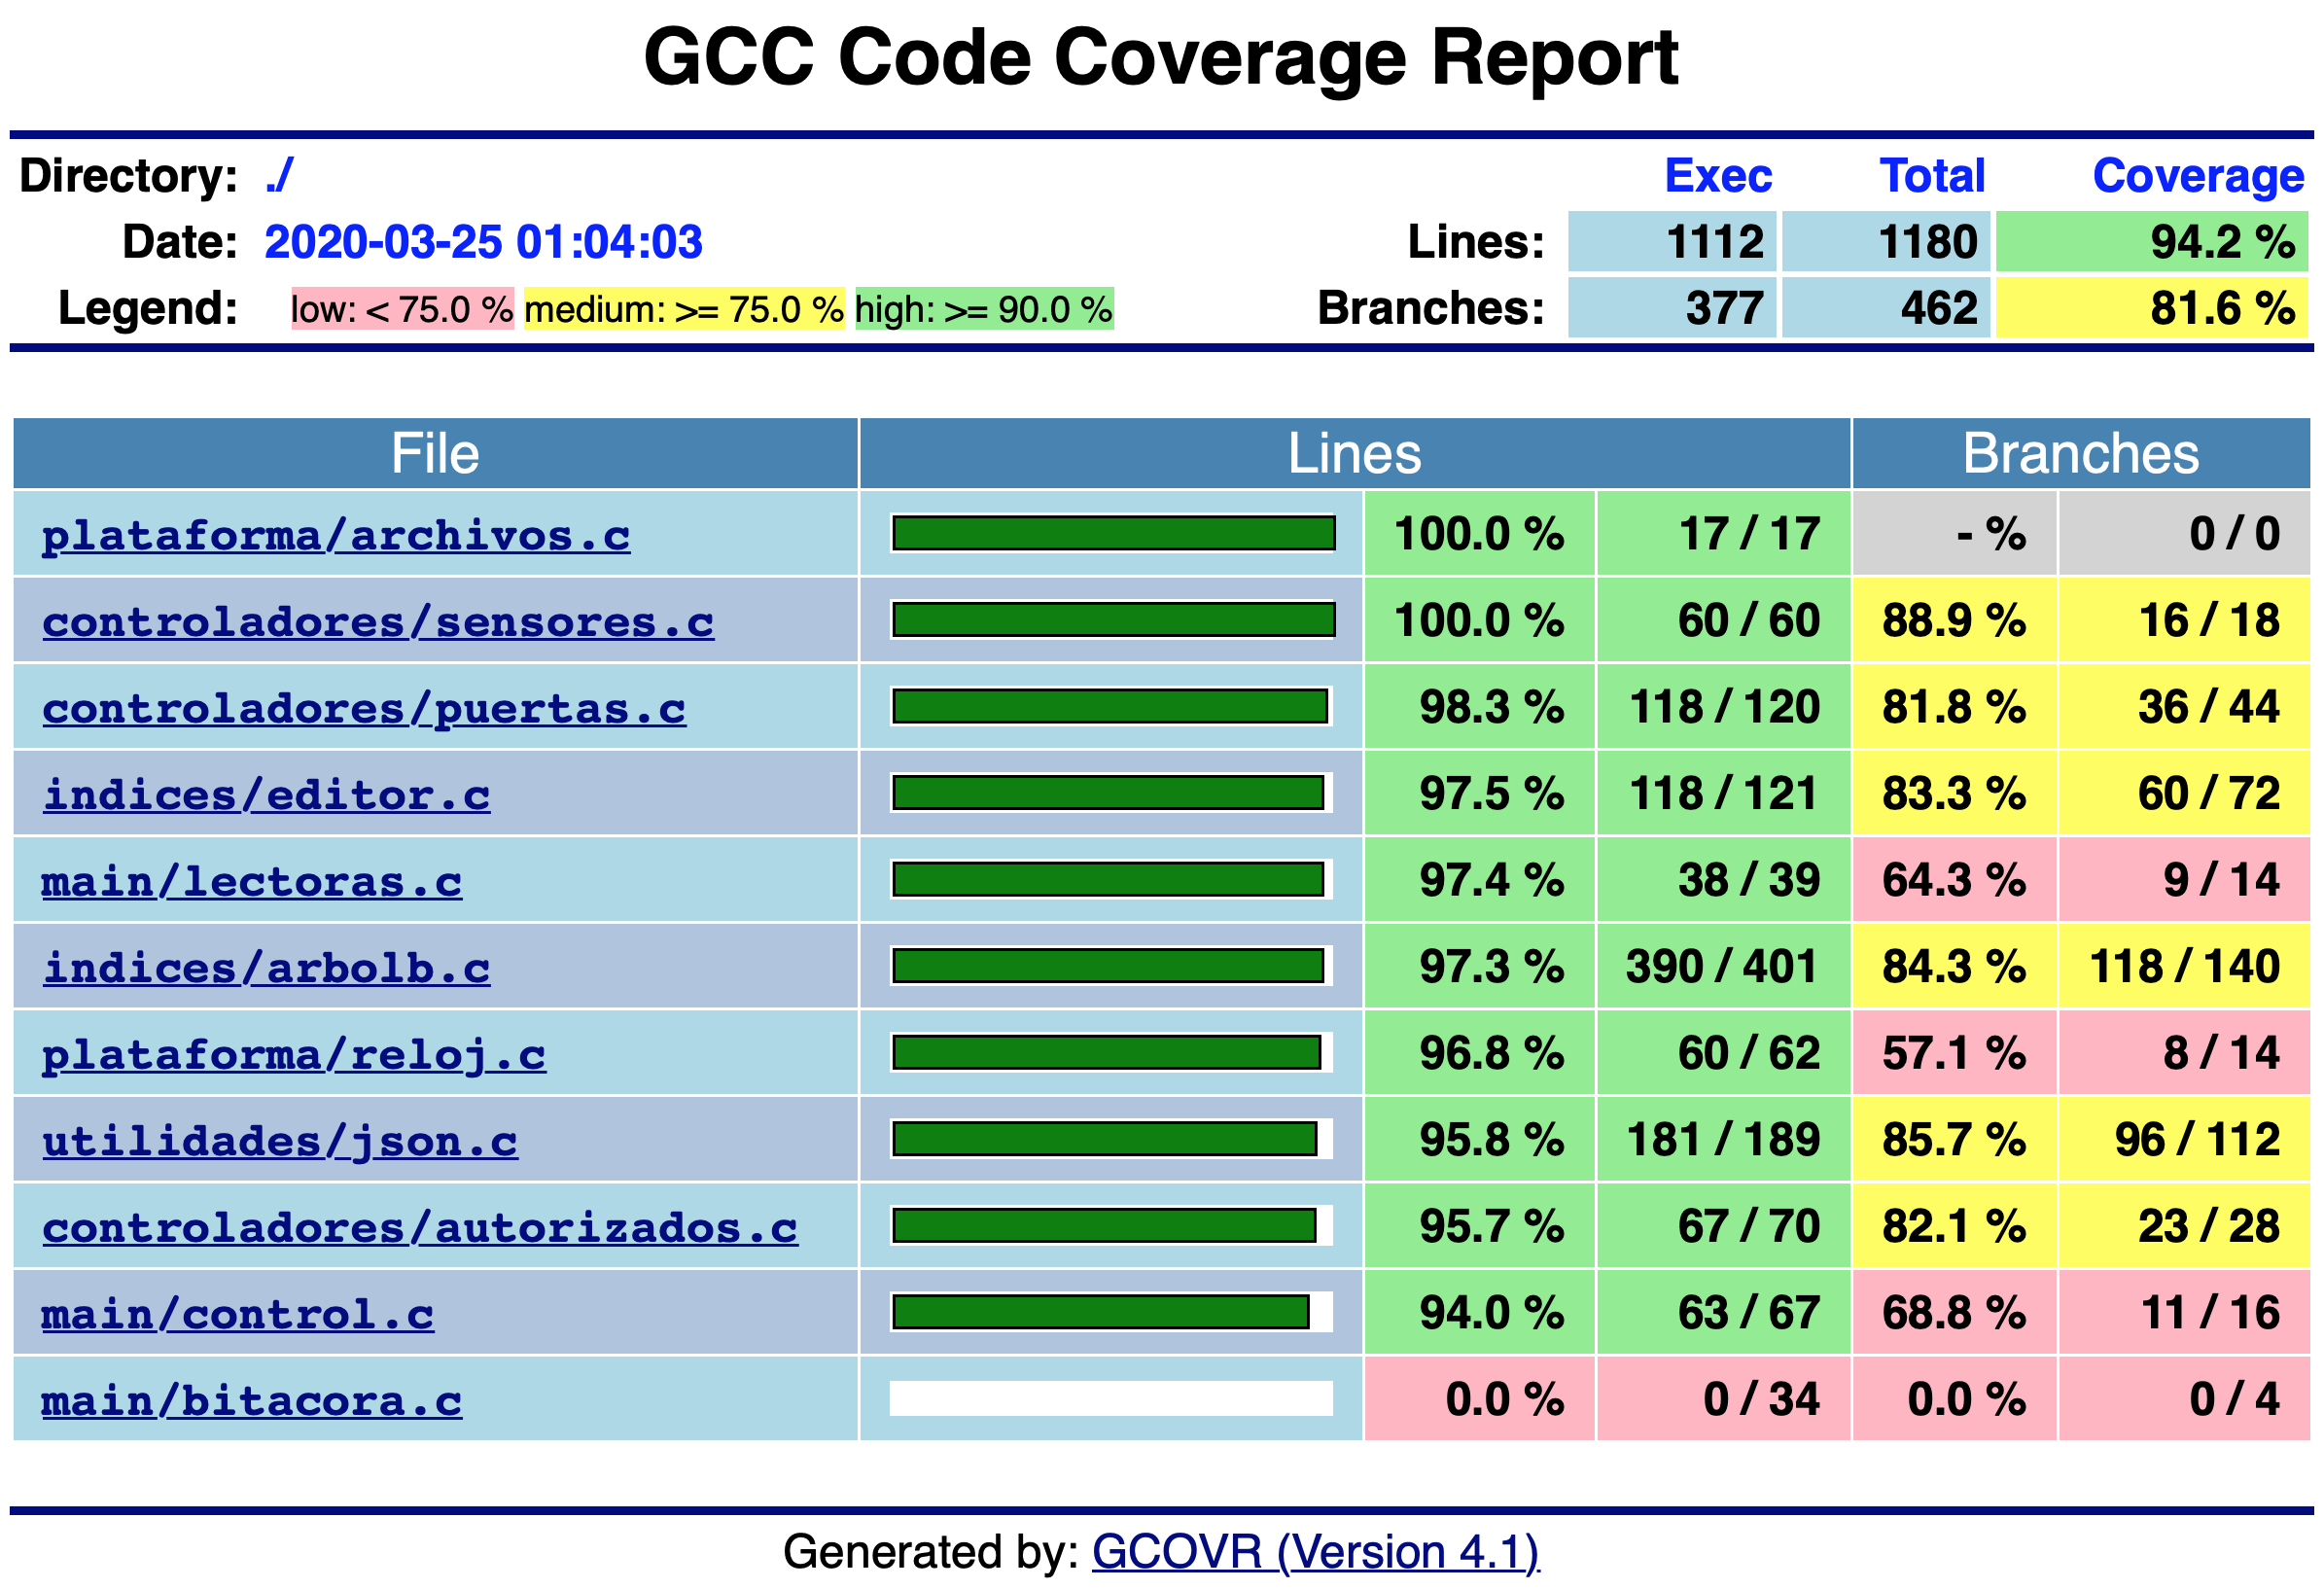
\includegraphics[width=\textwidth]{Figures/Cobertura.png}
	\caption[Informe con la cobertura de las pruebas]{Imagen con el informe de cobertura de las pruebas automatizadas efectuadas sobre el firmware.}
	\label{fig:Cobertura}
\end{figure}

Para dimensionar el esfuerzo realizado en la documentación y pruebas del código se utilizó la herramienta CLOC. Esta permite contabilizar las líneas de código fuente y las de comentarios para cada uno de los archivos. Aplicándola en forma separada para el código de producción y las pruebas automatizadas se obtuvieron los valores que se muestran en la tabla \ref{tab:MetricasFirmware}. Estos se pueden resumir en la siguiente afirmación: por cada diez líneas de código de producción se escribieron siete de documentación y cuatro de pruebas automatizadas.

\begin{table}[h]
	\centering
	\caption[Metricas de documentación y pruebas]{Tabla resumen con las métricas de documentación y pruebas obtenidas para el firmware desarrollado.}
	\begin{tabular}{l c c c c c }
		\toprule
		\textbf{Grupo} &
		\textbf{Tipo} &
		\textbf{Archivos} &
		\textbf{Código} &
		\textbf{Comentarios} &
		\textbf{Relación} \\
		\midrule
		\multirow[c]{2}{*}{Producción}
				& Cabeceras & 25 & 1078 & 2419 & 2,24 \\
				& Código C 	& 21 & 3770 & 1243 & 0,33 \\
		Pruebas & Código C 	& 11 & 1813 & 1010 & 0,56 \\
		\textbf{Totales} &		    & 	 & \textbf{6661} & \textbf{4672} & 0,\textbf{70}  \\
		\bottomrule
		\hline
	\end{tabular}
	\label{tab:MetricasFirmware}
\end{table}

\section{Resultado de las pruebas}
\label{sec:PruebasFirmware}

Los resultados de las pruebas en la placa electrónica, después de efectuar las correcciones mencionadas en las secciones \ref{sec:hardware} y \ref{sec:pruebasHW}, muestran un buen comportamiento del diseño, el cual se mostró estable durante todas las pruebas del firmware. En lo que respecta al firmware, por haber sido desarrollado utilizando la metodología TDD, el mismo cumplió con el comportamiento esperado sin necesidad de efectuar cambios. 

Es importante aclarar que las pruebas de aceptación del equipo no se ejecutaron en forma automática, ya que para ello es necesario el desarrollo de hardware específico que genere los estímulos y verifique las reacciones de la placa bajo prueba. Por esta razón estas pruebas se ejecutaron manualmente, siguiendo los guiones escritos en Gherkin que se mostraron en la sección \ref{sub:PruebasAceptacion}, y todas fueron completadas en forma exitosa por el equipo desarrollado. 





